\documentclass[11pt]{article}
\usepackage[utf8]{inputenc}
\usepackage[margin=1in]{geometry}
\usepackage{titling}
\usepackage{longtable}
\usepackage{array}
\usepackage{enumitem}
\usepackage{hyperref}
\usepackage{graphicx}
\usepackage{xcolor}
\usepackage{fancyhdr}
\usepackage{booktabs}

% Hyperlink setup
\hypersetup{
    colorlinks=true,
    linkcolor=blue,
    filecolor=magenta,      
    urlcolor=blue,
}

% Header/Footer
\pagestyle{fancy}
\fancyhf{}
\rhead{Team 7: Empowerment Farm}
\lhead{COP 3710 - Spring 2026}
\cfoot{\thepage}

\begin{document}

% --------------------------------------------------------------------------------
% TITLE PAGE
% --------------------------------------------------------------------------------
\begin{titlepage}
    \centering
    \vspace*{2cm}
    
    {\Huge \textbf{Partnership Proposal \& Needs Assessment}}
    
    \vspace{1.5cm}
    
    {\Large \textbf{COP 3710: Database Concepts}}
    
    \vspace{0.5cm}
    {\large Spring 2026}
    
    \vspace{2cm}
    
    \textbf{Submitted by Team 7:}
    
    \vspace{0.5cm}
    
    \begin{tabular}{ll}
        \textbf{Adil Zaben} & azaben8742@eagle.fgcu.edu \\
        \textbf{Sean Peppers} & speppers5329@eagle.fgcu.edu \\
        \textbf{Katharine Ringo} & karingo2009@eagle.fgcu.edu \\
    \end{tabular}
    
    \vspace{2cm}
    
    \textbf{One PDF containing:}
    \begin{itemize}
        \item Partner Confirmation Form
        \item Needs Assessment Meeting Notes
        \item Eagle Service Network (ESN) Registration
        \item Project Proposal
    \end{itemize}
    
    \vfill
    
    \textbf{Submission Date:} February 2, 2026
    
\end{titlepage}

\newpage

% --------------------------------------------------------------------------------
% PART A: PARTNERSHIP IDENTIFICATION
% --------------------------------------------------------------------------------
\section*{PART A: PARTNERSHIP IDENTIFICATION}

% --------------------------------------------------------------------------------
% 1. PARTNER SELECTION / CONFIRMATION FORM
% --------------------------------------------------------------------------------
\subsection*{1. Partner Confirmation Form}

\noindent\fbox{
    \begin{minipage}{0.95\textwidth}
        \begin{center}
            \textbf{\Large PARTNER CONFIRMATION FORM}\\
            COP 3710 - Database Project with Service Learning\\
            Spring 2026
        \end{center}
        
        \vspace{0.5cm}
        
        \textbf{\underline{STUDENT TEAM INFORMATION}}
        \begin{itemize}
            \item \textbf{Team Number:} 7
            \item \textbf{Team Members:}
            \begin{itemize}
                \item Adil Zaben (azaben8742@eagle.fgcu.edu)
                \item Sean Peppers (speppers5329@eagle.fgcu.edu)
                \item Katharine Ringo (karingo2009@eagle.fgcu.edu)
            \end{itemize}
        \end{itemize}
        
        \vspace{0.3cm}
        
        \textbf{\underline{COMMUNITY PARTNER INFORMATION}}
        \begin{itemize}
            \item \textbf{Organization Name:} Empowerment Farm
            \item \textbf{Contact Person:} Tiffany Lehman
            \item \textbf{Title/Position:} Founder/Executive Director
            \item \textbf{Email:} Tiffany@empowermentfarm.org
            \item \textbf{Phone:} 239-330-2777
        \end{itemize}
        
        \vspace{0.2cm}
        
        \textbf{Brief Description of Organization Mission:}
        \par
        Empowerment Farm is a non-profit dedicated to supporting their community through compassion and connection to the land and animals. They help provide our local area with inclusive, hands-on learning via applied education and work-based skills. Their "Common Ground" connections help uplift individuals of all abilities to build confidence. We will help develop a database to track their activities and give them a measurement of participation outcomes and experiences.
        
        \vspace{0.5cm}
        
        \textbf{\underline{CONFIRMATION}}
        \par
        By signing below, we confirm our partnership for the COP 3710 Database Project (Spring 2026). The student team will design and develop a database system to address the organization’s data management needs.
        
        \vspace{0.5cm}
        
        \begin{tabular}{p{8cm} p{6cm}}
            \textbf{Student Team Lead Signature:} & \textbf{Date:} Jan 28, 2026 \\
            \textit{Adil Zaben} & \\
            \\
            \textbf{Community Partner Signature:} & \textbf{Date:} Jan 28, 2026 \\
            \textit{Tiffany Lehman} & \\
        \end{tabular}
    \end{minipage}
}

\vspace{0.5cm}

\begin{center}
    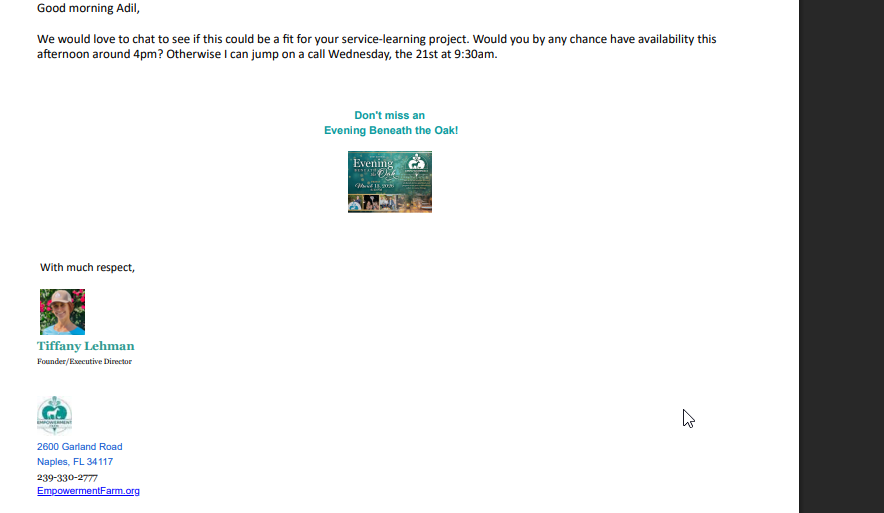
\includegraphics[width=0.9\textwidth]{proof_of_meeting.png}
    \par\textit{Figure 3: Email Confirmation of Partnership and Initial Meeting}
\end{center}

\newpage

% --------------------------------------------------------------------------------
% 2. NEEDS ASSESSMENT MEETING NOTES
% --------------------------------------------------------------------------------
\subsection*{2. Needs Assessment Meeting Notes}

\begin{tabular}{|l|p{10cm}|}
    \hline
    \textbf{Date:} & January 28, 2026 \\ \hline
    \textbf{Mode:} & Virtual Meeting (Phone/Email follow-up) \\ \hline
    \textbf{Attendees:} & Adil Zaben (Team Lead), Tiffany Lehman (Executive Director) \\ \hline
    \textbf{Subject:} & Initial Needs Assessment \& Project Scope Definition \\ \hline
\end{tabular}

\vspace{0.5cm}

\subsubsection*{Current Challenges}
During our discussion, Tiffany highlighted several key challenges with Empowerment Farm's current data management:
\begin{itemize}
    \item \textbf{Ad-hoc Data Collection:} Currently, data is collected via disparate paper forms or isolated spreadsheets (e.g., Google Sheets), making it difficult to visualize trends over time.
    \item \textbf{Measuring "Soft" Outcomes:} A core challenge is quantifying the therapeutic benefits of the farm (e.g., "felt more calm", "felt connected") effectively for grant reporting without clinical tools.
    \item \textbf{Privacy Concerns:} The organization operates under a "Labels Stop at the Gate" philosophy. They need to track outcomes without necessarily requiring intrusive diagnostic labels or mandatory account creation for every casual visitor.
    \item \textbf{Grant Reporting:} Compiling data for grant applications is currently a manual, time-consuming process involving tallying paper records or merging spreadsheets.
\end{itemize}

\subsubsection*{Identified Data Needs}
We identified the following core data entities and requirements:
\begin{itemize}
    \item \textbf{Program Tracking:} A catalog of all offerings (e.g., \textit{Cow Yoga, Tuesday Night Tuck-In, Open Farm, Educational Field Trips}).
    \item \textbf{Participant Feedback (The "Survey"):} A streamlined digital way to capture post-activity feedback. Key metrics identified include:
    \begin{itemize}
        \item Presence/Engagement
        \item Connection to Others
        \item Connection to Nature/Animals
        \item Calmness/Stress Reduction
        \item Learning Intent
    \end{itemize}
    \item \textbf{Farm Zones \& Animals:} Tracking which farm areas (e.g., \textit{Pollinator Garden, Main Barnyard}) and animals are most utilized in therapy sessions to justify resource allocation.
    \item \textbf{Constituent Profiles:} A secure way to store contact info for recurring volunteers and students, while allowing one-time visitors to remain relatively anonymous (tracking only age range/demographics).
\end{itemize}

\subsubsection*{Future Goals}
The immediate goal is a working "Impact Dashboard" that Tiffany can open to see real-time stats like "85\% of participants reported reduced stress this month." Future goals include tracking longitudinal progress of specific students over multiple sessions.

\vspace{0.5cm}
\begin{center}
    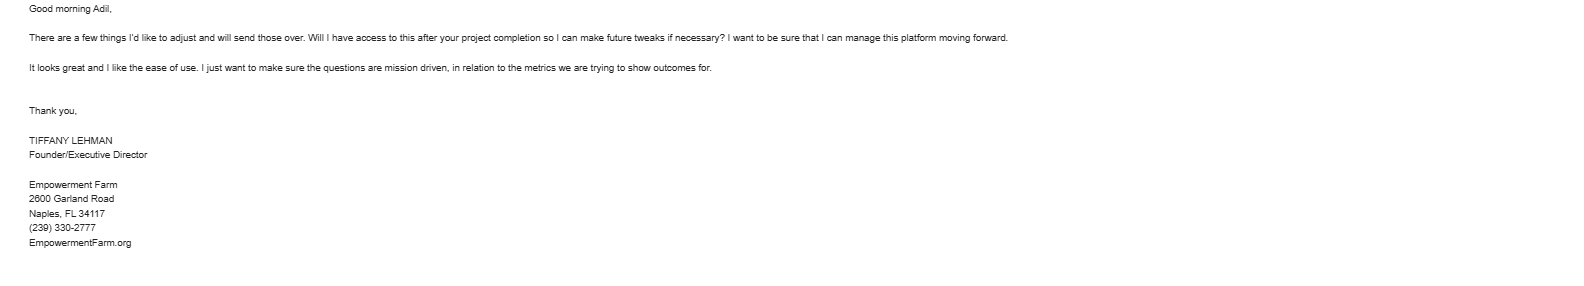
\includegraphics[width=0.9\textwidth]{requirement_tweaks.png}
    \par\textit{Figure 4: Notes on Requirement Refinements and Data Needs}
\end{center}

\newpage

% --------------------------------------------------------------------------------
% 3. EAGLE SERVICE NETWORK REGISTRATION
% --------------------------------------------------------------------------------
\subsection*{3. Eagle Service Network (ESN) Registration}

\begin{center}
    \vspace{1cm}
    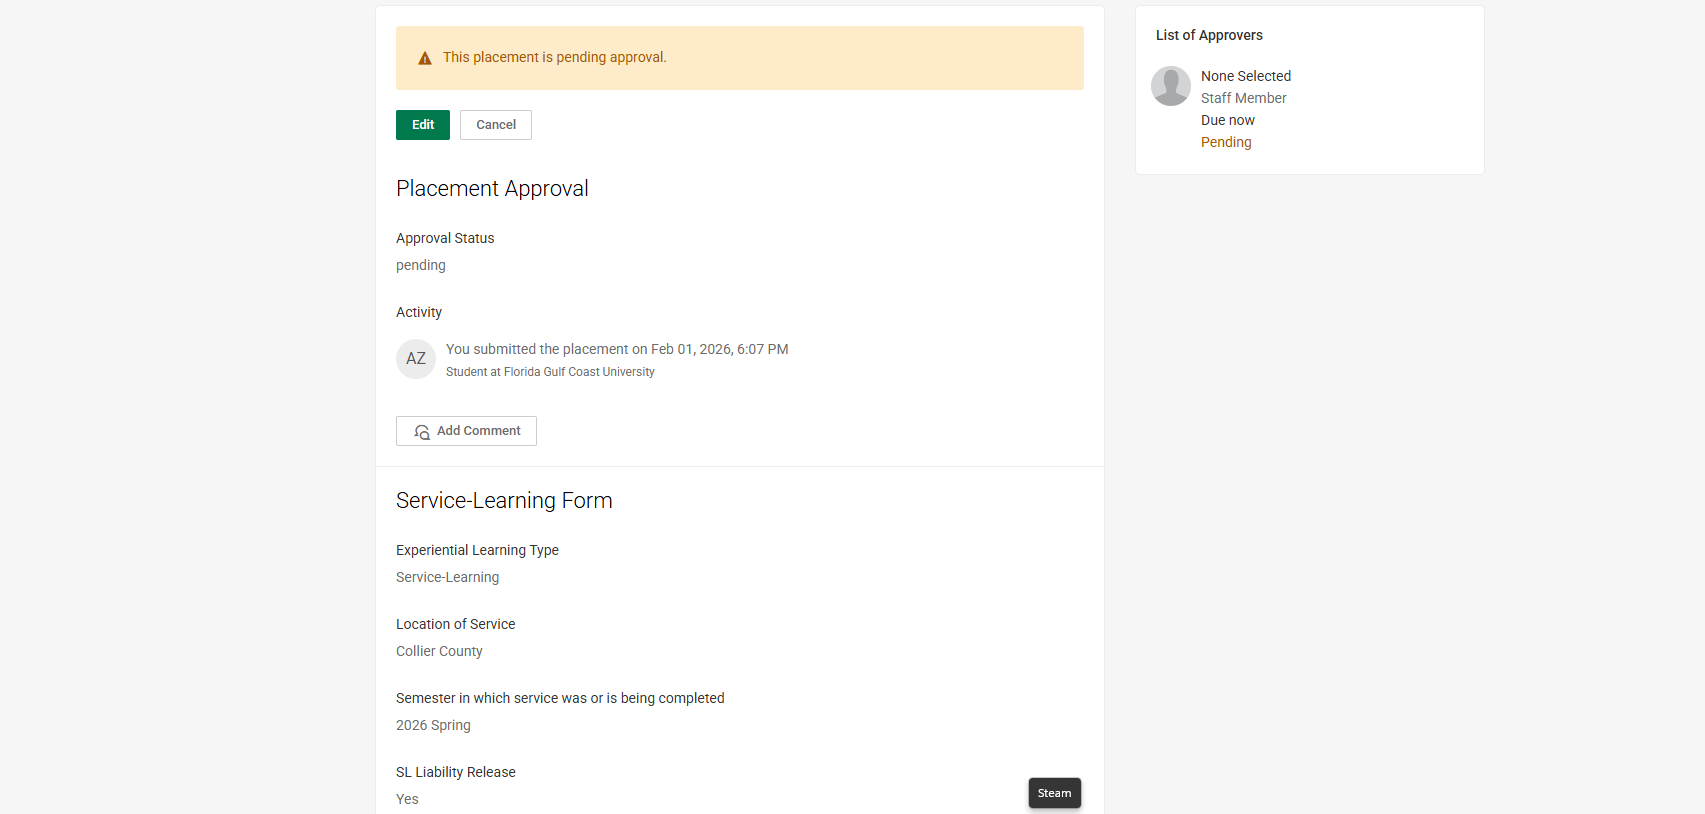
\includegraphics[width=1.0\textwidth]{lr_form_pending.png}
    
    \vspace{0.5cm}
    \textit{Figure 1: Service Learning Registration (Pending Approval)}
\end{center}

\newpage

% --------------------------------------------------------------------------------
% PART B: PROJECT PROPOSAL
% --------------------------------------------------------------------------------
\section*{PART B: PROJECT PROPOSAL}

\subsection*{1. Project Objective}
The primary objective of this project is to design and develop a secure, web-based \textbf{Therapeutic Outcomes Database} for Empowerment Farm. This system will replace ad-hoc data collection methods with a centralized platform that tracks program participation and measures the "soft metrics" of farm-based therapy (e.g., calmness, connection, engagement). 

By digitizing this data, the project will directly benefit the organization by:
\begin{itemize}
    \item Automating the generation of impact reports needed for grant funding.
    \item Providing insights into which programs (e.g., Cow Yoga vs. Field Trips) yield the highest therapeutic engagement.
    \item Adhering to the "Labels Stop at the Gate" philosophy by allowing for anonymous yet demographically significant data collection.
\end{itemize}

\subsection*{2. Community Partner Overview}
\textbf{Empowerment Farm} is a non-profit organization located in Naples, FL, founded by Tiffany Lehman. 
\begin{itemize}
    \item \textbf{Mission:} To support the community through compassion and connection to the land and animals.
    \item \textbf{Services:} They offer inclusivity-focused programs such as \textit{Cow Yoga}, \textit{Tuesday Night Tuck-In}, and \textit{educational field trips} that provide hands-on learning and work-based skills.
    \item \textbf{Target Population:} Individuals of all abilities, including local youth, families, and those seeking therapeutic connection with nature.
    \item \textbf{Current Data Challenges:} The lack of a centralized database makes it difficult to track repeat visitors or quantify the subjective benefits of their programs, which is critical for their non-profit status and funding.
\end{itemize}

\subsection*{3. Scope of the Project}
This project will focus on the following agreed-upon deliverables:

\textbf{In Scope:}
\begin{itemize}
    \item \textbf{Database Schema Design:} Creating a normalized Relational Database Management System (RDBMS) to store data on constituents, farm animals, farm zones, programs, and experiences.
    \item \textbf{Survey/Feedback Module:} A " kiosk-style" or mobile-friendly web form for participants to log their post-activity feedback (Likert scale 1-3 for calmness, connection, etc.).
    \item \textbf{Constituent Management:} A system to manage profiles for staff, volunteers, and recurring students, with support for anonymous demographic tracking for one-time visitors.
    \item \textbf{Impact Dashboard:} SQL views and queries to aggregate data (e.g., "Average Calmness Score by Activity Type").
\end{itemize}

\textbf{Out of Scope:}
\begin{itemize}
    \item \textbf{Payment Processing:} We will not handle ticket sales or donation processing within this database; financial transactions remain external.
    \item \textbf{Clinical Medical Records (EMR):} To maintain the "Labels Stop at the Gate" mission, we will not store detailed medical diagnoses or clinical history (HIPAA compliance for medical records is not required for this specific scope).
\end{itemize}

\subsection*{4. Dataset Description}
The database will manage a variety of real-world customized data types reflecting the farm's operations:

\begin{itemize}
    \item \textbf{Constituents:} Data on people involved (Staff, Volunteers, Students). Includes \textit{Names, Emails, Role Types, and Age Ranges}.
    \item \textbf{Farm Assets:}
    \begin{itemize}
        \item \textit{Animals:} Species, Breed, Name (e.g., "Goats", "Cows"), and "Is Therapy Animal" flags.
        \item \textit{Farm Zones:} Physical locations like "Pollinator Garden", "Main Barnyard", "Yoga Pasture".
    \end{itemize}
    \item \textbf{Program Catalog:} Metadata for events like "Cow Yoga" or "Seedlings for Spring," including descriptions and costs.
    \item \textbf{Experiences \& Surveys:} The core transactional data. This includes attendance records and survey responses measuring specific outcomes:
    \begin{itemize}
        \item \textit{Quantitative:} Scores (1-3) for "Is Present/Engaged", "Connection to Others", "Connection to Nature".
        \item \textit{Qualitative:} Text fields for "Standout Moments" or "Referral Sources".
    \end{itemize}
\end{itemize}
    
    \begin{center}
        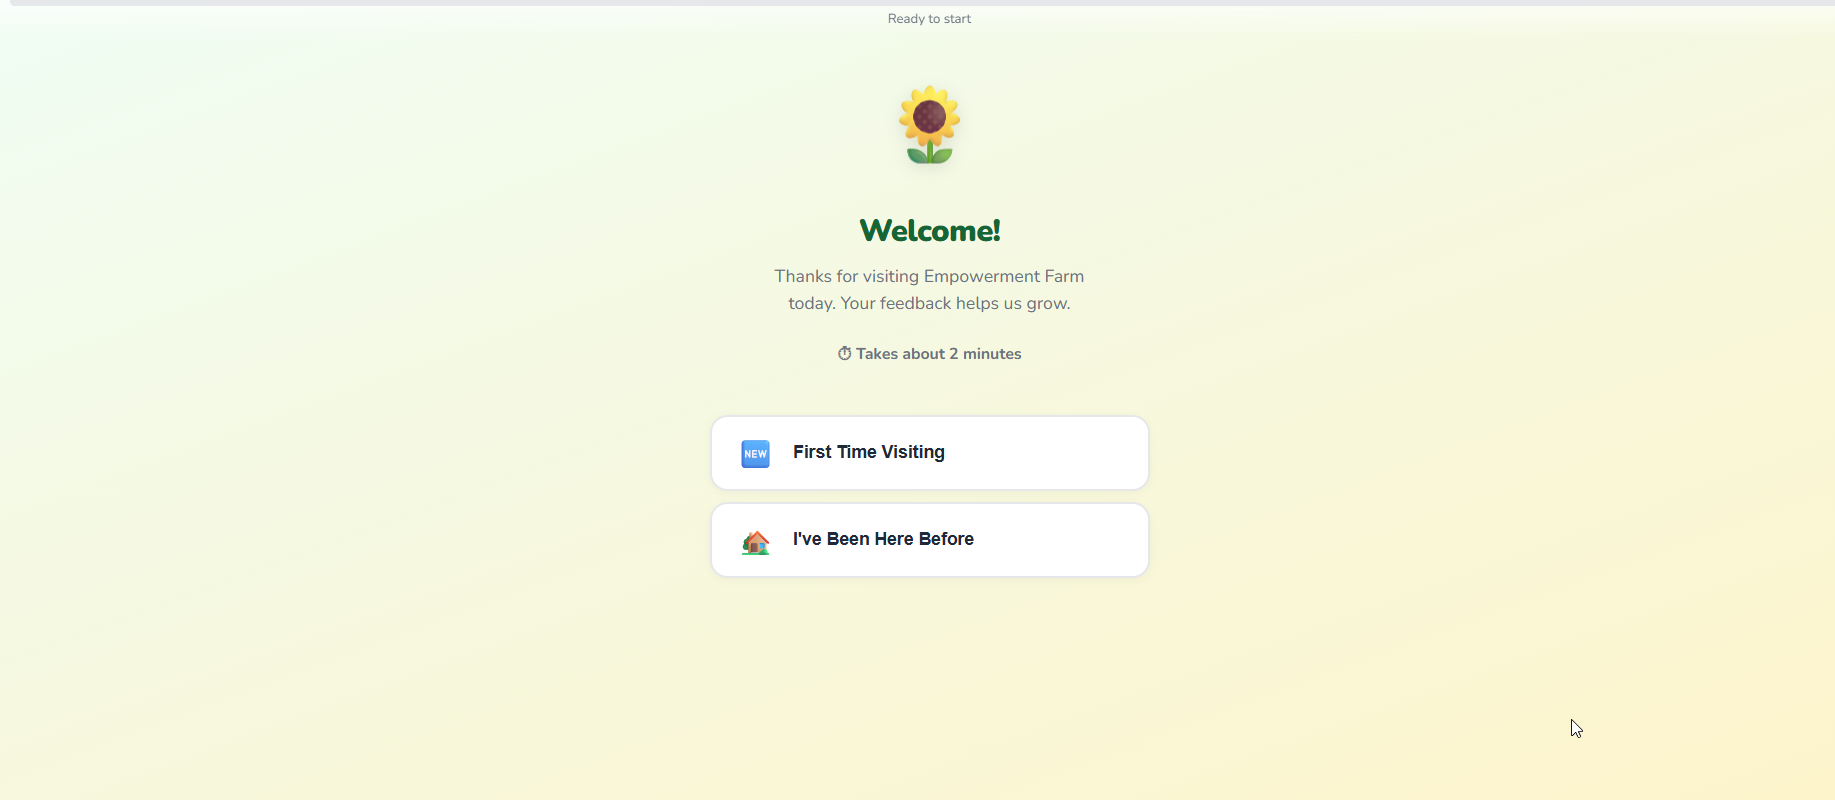
\includegraphics[width=0.7\textwidth]{emp_farm_survey.png}
        \par\textit{Figure 2: Survey Tool Interface}
    \end{center}

\subsection*{5. Impact Statement}
This database system will fundamentally improve Empowerment Farm's operations by moving them from anecdotal evidence to data-driven decision-making. 
\begin{itemize}
    \item \textbf{Operations:} Staff can easily schedule volunteers or see which farm zones are most utilized.
    \item \textbf{Service Delivery:} By analyzing feedback scores, Tiffany can identify that, for example, "Cow Yoga" produces higher "Calmness" scores than other activities, allowing them to optimize their schedule for maximum therapeutic benefit.
    \item \textbf{Sustainability:} The ability to generate professional data reports will significantly strengthen grant applications, ensuring the farm can secure funding to continue its mission.
\end{itemize}

\subsection*{6. Partner Approval}
\textit{Refer to Part A (Section 1) for the signed Partner Confirmation Form. Additionally, email correspondence dated Jan 26, 2026, from Tiffany Lehman ("Awesome. Thank you!!") confirms approval of the project direction to build a database for tracking farm outcomes.}

\end{document}
